\chapter{Performance Evaluation Results}

\section{Noise in Simulated Experiments}

To quantify the amount of noise in the images after the computation of the \gls{bold}, we use the \gls{cnr} and \gls{snr} \cite{welvaert2013definition}. Note that the precision of the calculations depends on the noise present in the images. Therefore, the performance is expected to decrease as the amount of noise increases and the signals from active and inactive voxels are more difficult to differentiate.

For each of the 2 true maps considered and each of the 16 order combinations $(P,Q)$ for the $ARMA$ model to generate noise, 50 different \gls{bold} responses were generated, resulting in 1600 simulated \gls{fmri} experiments in total. A voxel-wise computation of the \gls{cnr} and \gls{snr} was made for all of them. See Figures \ref{fig:cnrsnr} for their numerical distributions. Additionally, Figures \ref{fig:snr2DSpatial} and \ref{fig:cnr2DSpatial} present the spatial distributions of the \gls{snr} and \gls{cnr} values in the \gls{2d} maps, respectively. Although it is not presented, the spatial distributions of the \gls{snr} and \gls{cnr} values in the \gls{3d} maps are expected to observe a similar behavior.

\begin{figure}[htbp!]
\centering
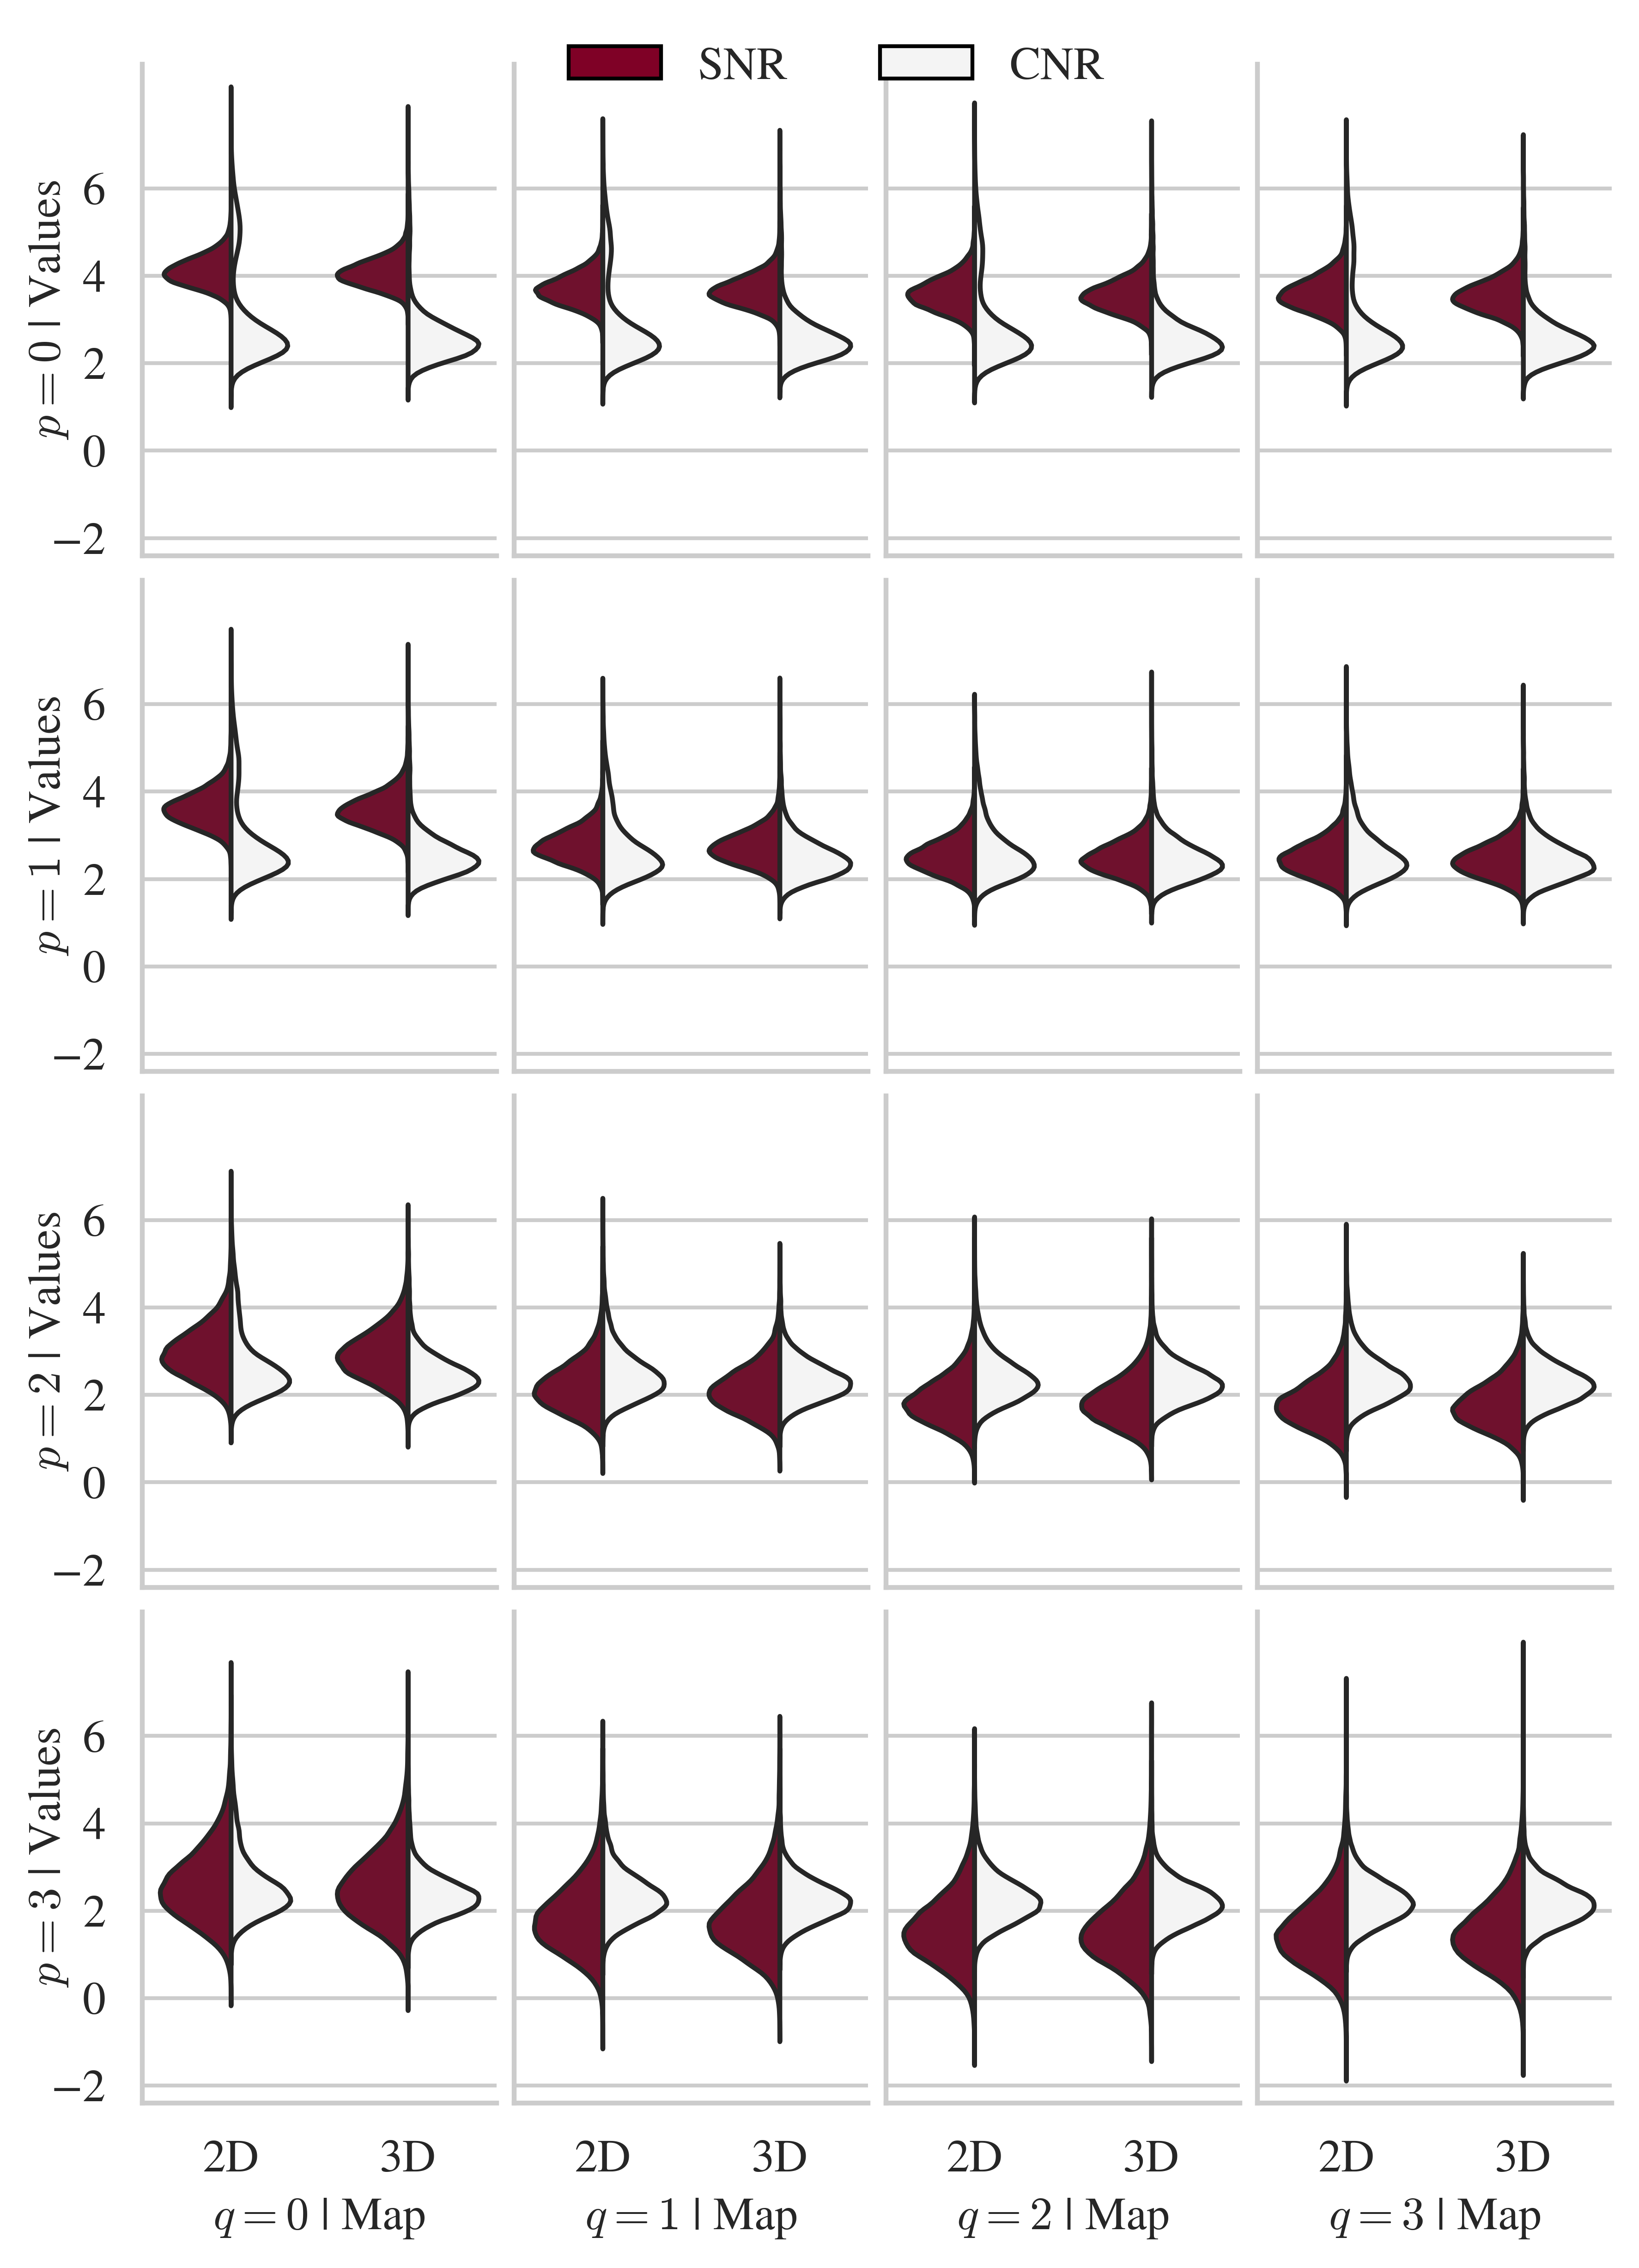
\includegraphics{images/cnrsnr.png}
\caption{Numerical Distribution of the Voxel-Wise \gls{snr} and \gls{cnr} Values}
\label{fig:cnrsnr}
\end{figure}

\begin{figure}[htbp!]
\centering
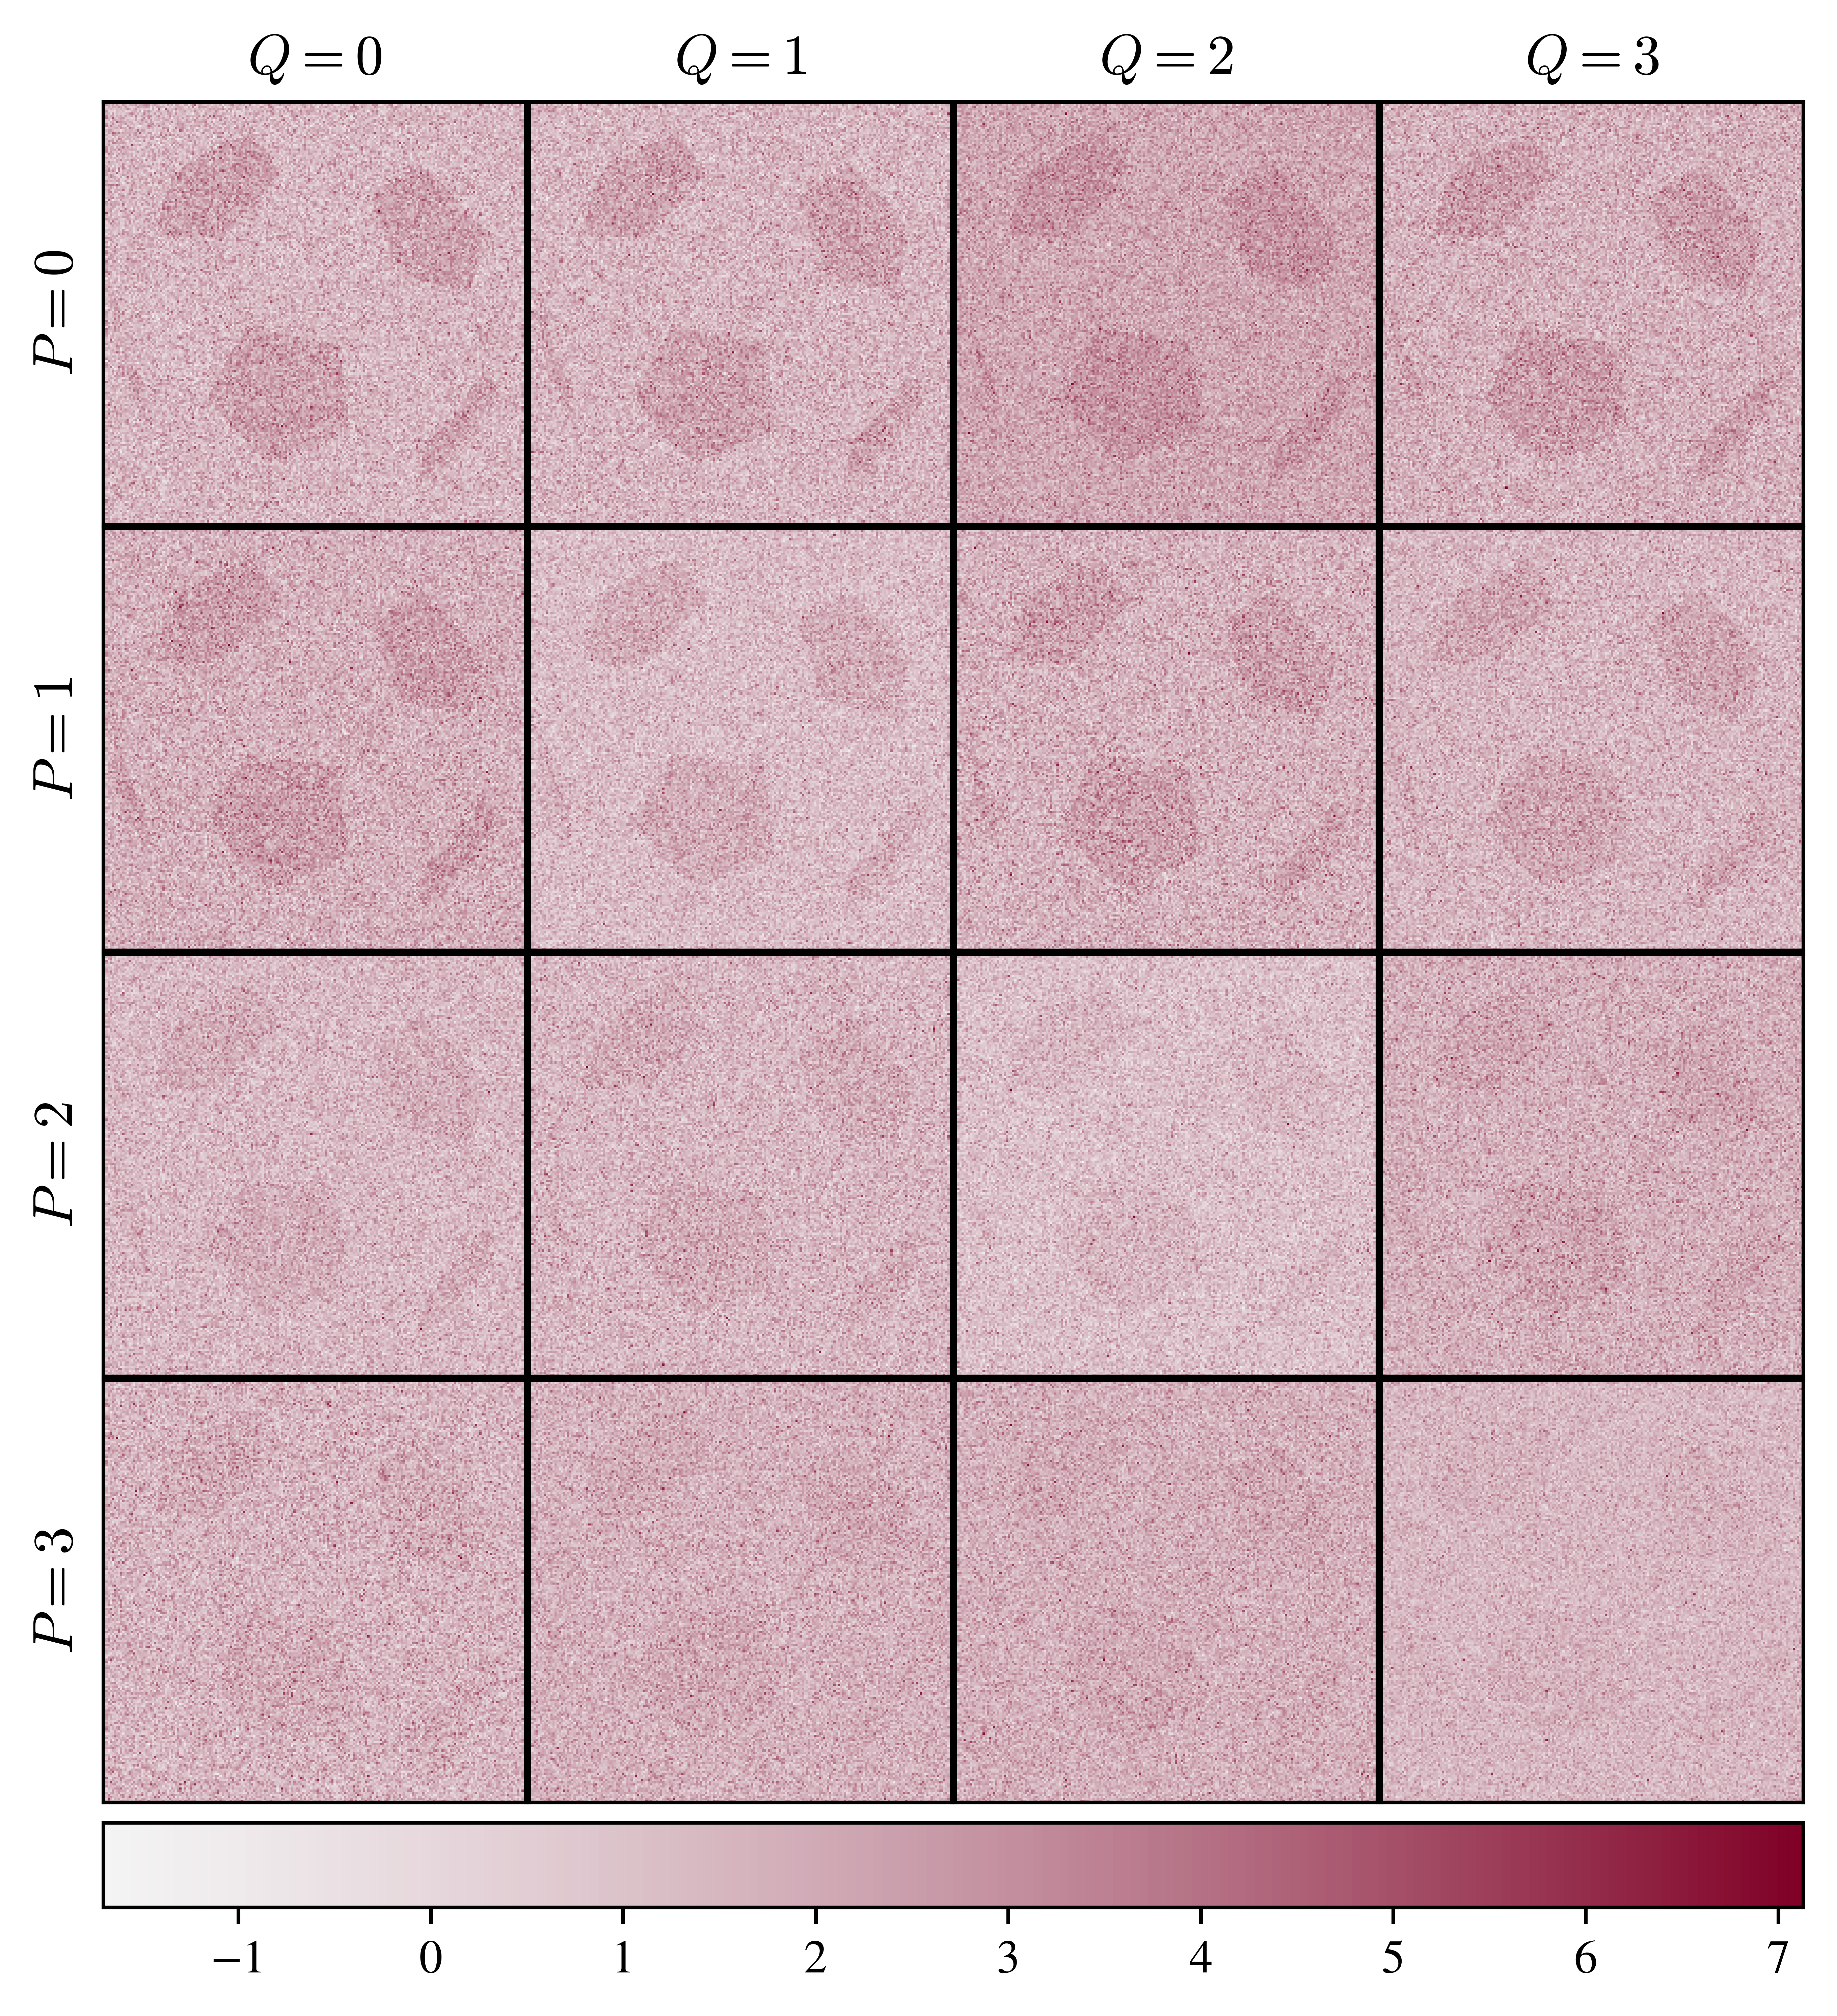
\includegraphics{images/snr2D_Spatial.png}
\caption{Spatial Distribution of the \gls{snr} Values in \gls{2d} Map}
\label{fig:snr2DSpatial}
\end{figure}

\begin{figure}[htbp!]
\centering
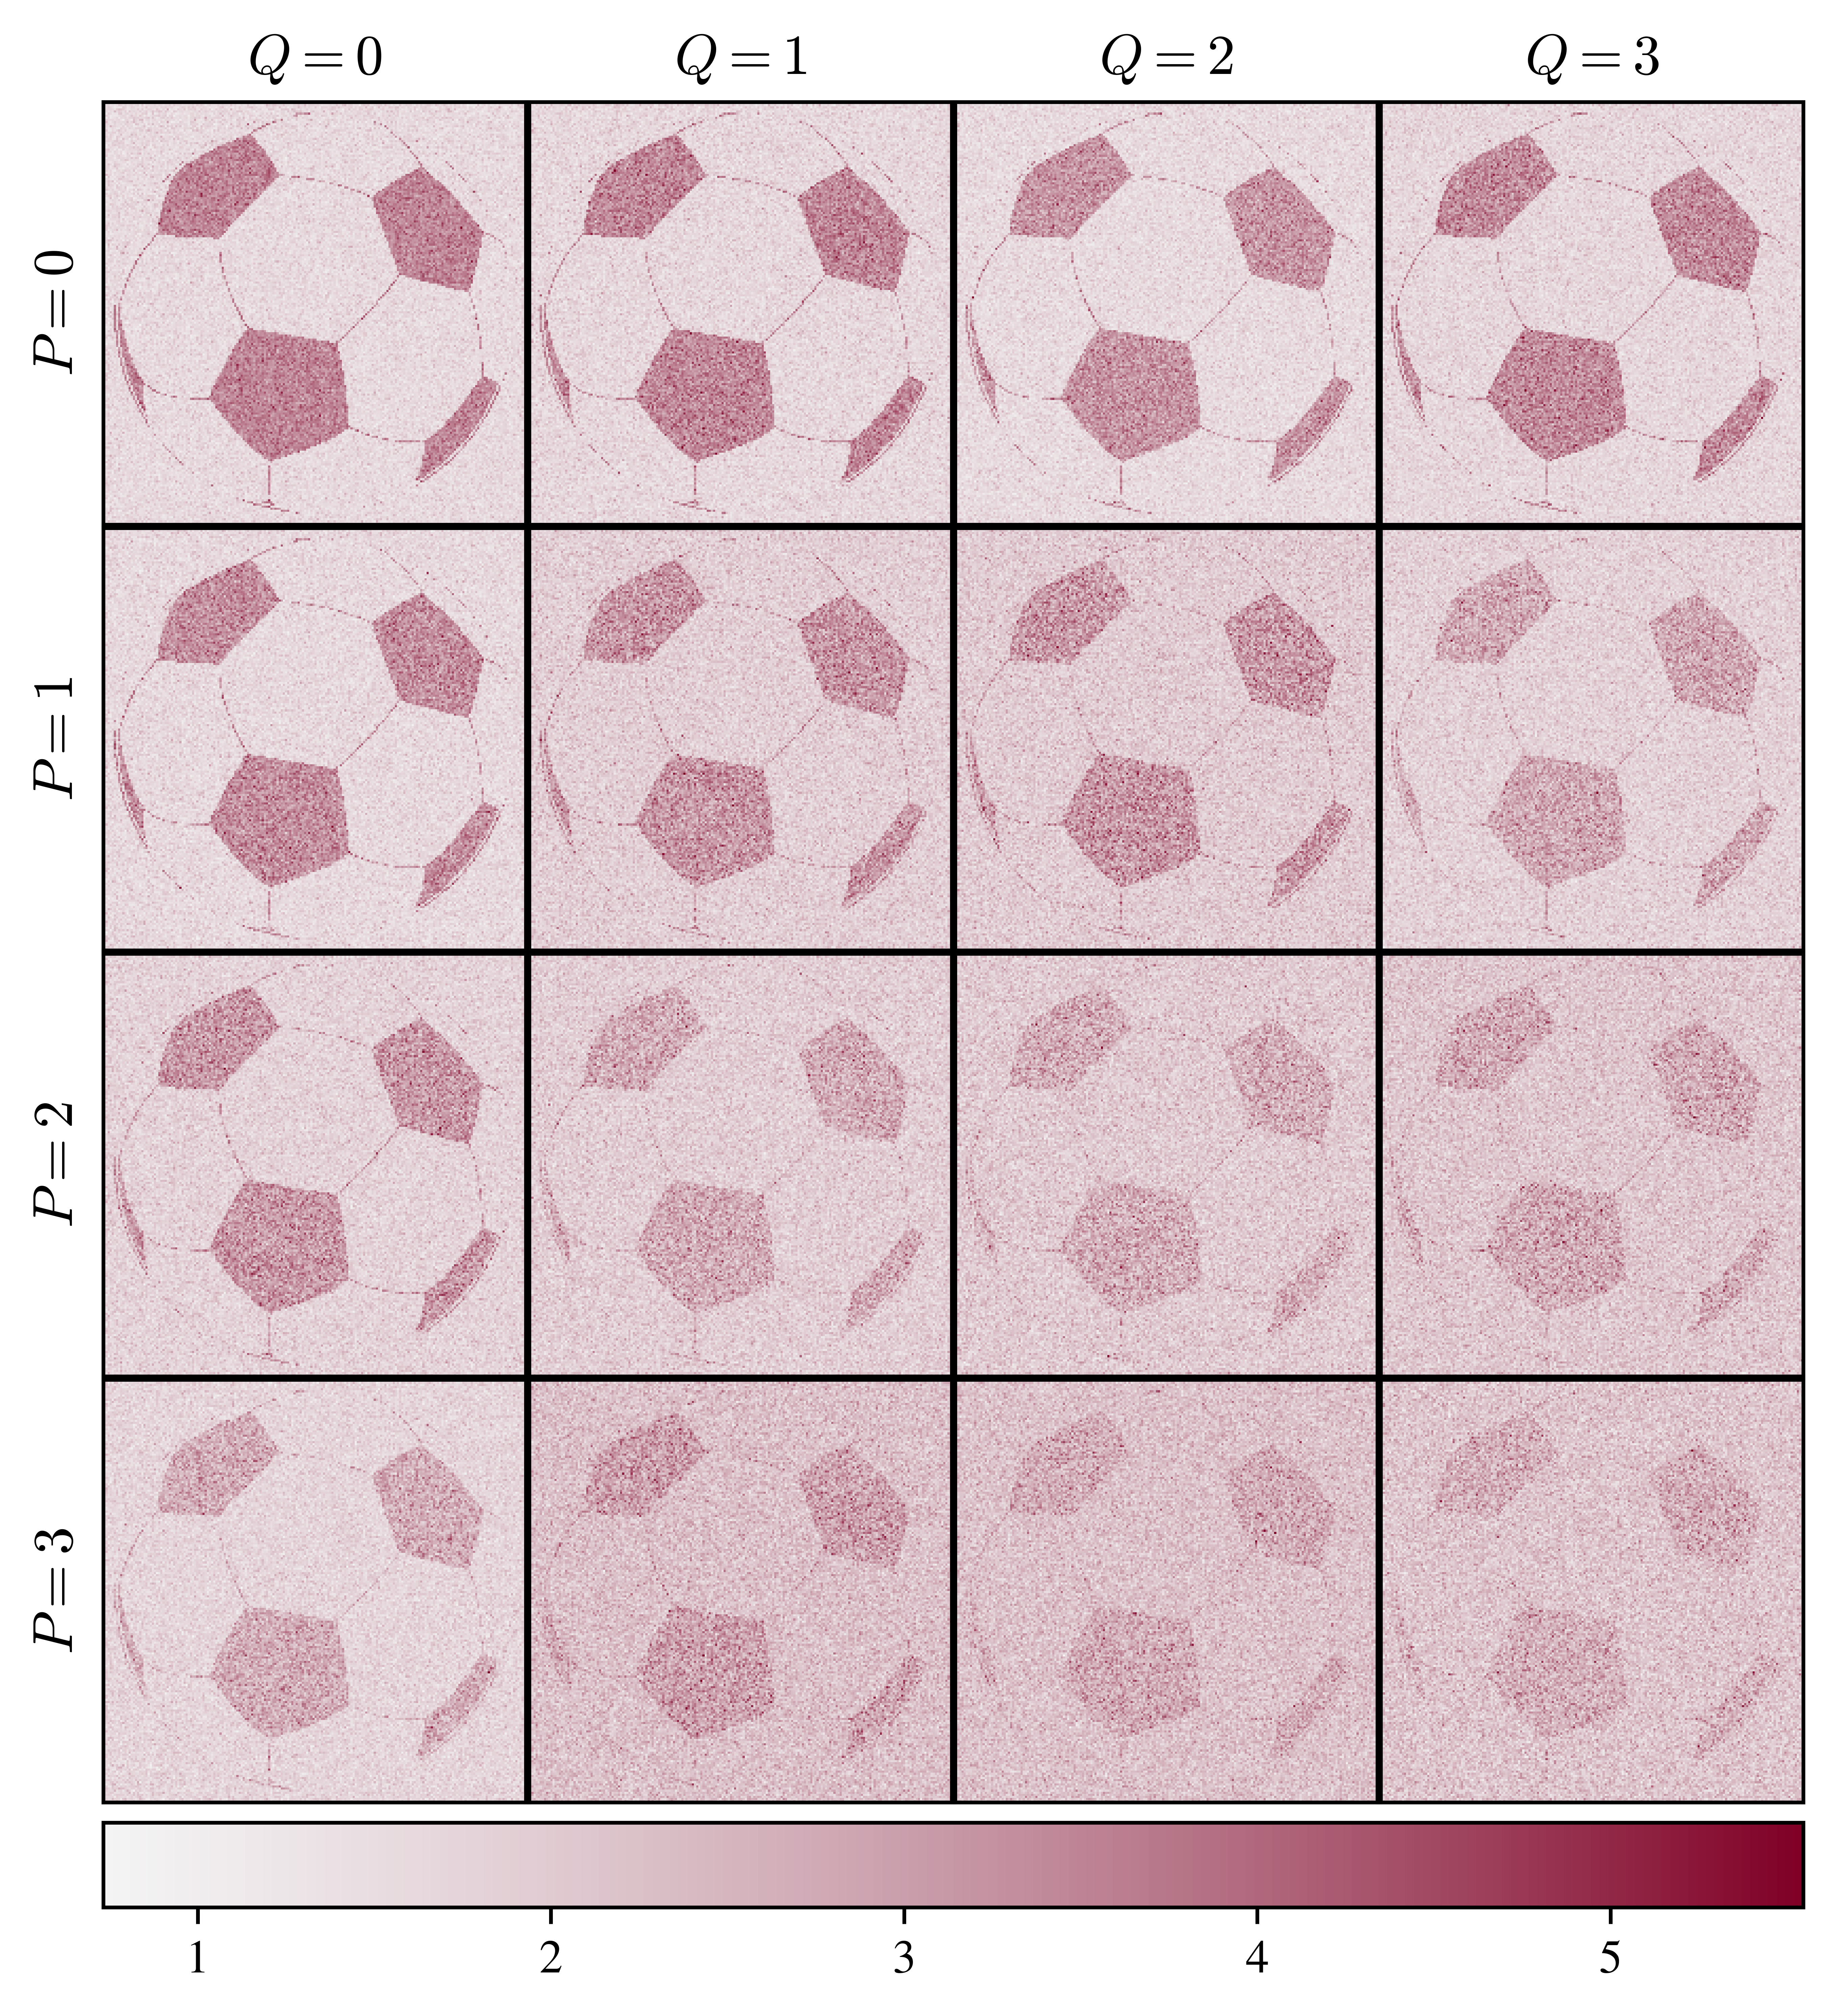
\includegraphics{images/cnr2D_Spatial.png}
\caption{Spatial Distribution of the \gls{cnr} Values in \gls{2d} Map}
\label{fig:cnr2DSpatial}
\end{figure}

\newpage

Note from Figure \ref{fig:cnrsnr} that the \gls{snr} and \gls{snr} values decrease as the values of $P$ or $Q$ increase, however, we can see that a change in the value of $P$ has a greater impact on the change of the \gls{snr} values. Additionally, we can see that the behavior of the \gls{snr} values does not change within the two maps. In contrast, the behavior of the \gls{cnr} values change in the two maps. Note that for the \gls{2d} map, the distribution of the \gls{cnr} for low values of $P$ and $Q$ can be interpreted as bimodal. This is because the number of active voxels in the \gls{2d} map is higher than in the \gls{3d} map, and active voxels have more contrast than inactive voxels. Finally, note that in both maps, for higher values of $P$ and $Q$, the \gls{snr} appears to be more distributed while the \gls{snr} appears to be less distributed. Finally, note from Figures \ref{fig:snr2DSpatial} and \ref{fig:cnr2DSpatial} that the \gls{snr} and \gls{cnr} values in our simulated \gls{fmri} experiment range from -2 to 7 and from 0 to 6, respectively. In both the \gls{snr} and \gls{cnr}, the active voxels are more difficult to visually differentiate as the values of $P$ and $Q$ increase.

\section{Example of the Procedure}

\section{Performance Metrics}

The performance of the \gls{bfast} algorithm was evaluated by comparing the final activated map with the true activation map using:

\begin{itemize}
\item \gls{ji}: Similarity between the two maps.
\item \gls{fpr}: Ratio of the voxels marked as activated that are not really active and the total number of inactive voxels.
\item \gls{poa} Error: Difference in the percentage of active voxels between both maps.
\end{itemize}

See Tables \ref{tab:perfSum} for the summary of these performance metrics.

\begin{table}[htbp!]
\centering
\caption{Performance Metrics Summary}
\begin{tabular}{cccccccccc}
\cline{5-10}
&&&& \multicolumn{3}{c}{\textbf{\gls{2d} Map}} & \multicolumn{3}{c}{\textbf{\gls{3d} Map}} \\ \hline
\textbf{P} & \textbf{Q} & \textbf{\gls{snr}} & \textbf{\gls{cnr}} & \gls{ji} & \gls{fpr} & \gls{poa} Error & \gls{ji} & \gls{fpr} & \gls{poa} Error \\ \hline
\multirow{4}{*}{0} & 0 & 4.0636 & 2.8250 & 0.9256 & 0.0078 & -0.2750 & 0.7677 & 0.0046 & -0.1450 \\
 & 1 & 3.6608 & 2.7607 & 0.8925 & 0.0180 & 0.5775 & 0.7249 & 0.0068 & 0.0425 \\
 & 2 & 3.5568 & 2.7367 & 0.8754 & 0.0227 & 0.9200 & 0.6796 & 0.0086 & 0.1150 \\
 & 3 & 3.5460 & 2.7310 & 0.8695 & 0.0244 & 1.0575 & 0.6767 & 0.0082 & 0.0425 \\ \hline
\multirow{4}{*}{1} & 0 & 3.5770 & 2.7364 & 0.8794 & 0.0222 & 0.9325 & 0.6741 & 0.0092 & 0.1975 \\
 & 1 & 2.7336 & 2.5914 & 0.8509 & 0.0299 & 1.4600 & 0.6468 & 0.0108 & 0.3125 \\
 & 2 & 2.4935 & 2.5298 & 0.8488 & 0.0308 & 1.5375 & 0.6410 & 0.0116 & 0.4025 \\
 & 3 & 2.4497 & 2.5164 & 0.8533 & 0.0292 & 1.4125 & 0.6757 & 0.0099 & 0.3100 \\ \hline
\multirow{4}{*}{2} & 0 & 2.9354 & 2.5817 & 0.8685 & 0.0240 & 0.9700 & 0.6979 & 0.0083 & 0.1600 \\
 & 1 & 2.1446 & 2.4047 & 0.8648 & 0.0267 & 1.2900 & 0.6566 & 0.0108 & 0.3575 \\
 & 2 & 1.8597 & 2.3326 & 0.8578 & 0.0284 & 1.3950 & 0.6909 & 0.0079 & 0.0550 \\
 & 3 & 1.7892 & 2.3115 & 0.8581 & 0.0283 & 1.3750 & 0.6859 & 0.0081 & 0.0775 \\ \hline
\multirow{4}{*}{3} & 0 & 2.5601 & 2.4581 & 0.8932 & 0.0174 & 0.5075 & 0.7297 & 0.0065 & 0.0125 \\
 & 1 & 1.8244 & 2.2855 & 0.8882 & 0.0185 & 0.5750 & 0.7194 & 0.0067 & 0.0000 \\
 & 2 & 1.5739 & 2.2153 & 0.8837 & 0.0200 & 0.7000 & 0.7167 & 0.0074 & 0.1075 \\
 & 3 & 1.5132 & 2.1919 & 0.8793 & 0.0213 & 0.8025 & 0.7092 & 0.0066 & -0.0600 \\ \hline
\end{tabular}
\label{tab:perfSum}
\end{table}